\documentclass[landscape]{foils}
\usepackage{graphicx,color,amsmath,amssymb,latexsym,enumerate}

\topmargin-2cm
\leftmargin-1cm
%%\voffset-1.5cm
%%\hoffset.5cm
%\textwidth25cm
%\parindent0pt
\textheight18cm

\MyLogo{Discrete Volume Computations for Polyhedra \quad 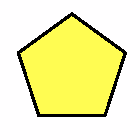
\includegraphics[viewport= 0 16 100 100, height=16pt]{pentagon} \ Matthias Beck}
\leftheader{}
\rightheader{}

\def\MB{M\hspace{-6pt}B }
\def\mybullet{\green $\blacktriangleright$ \black}

\newcounter{frozenpage}
\def\freezepage{
  \setcounter{frozenpage}{\thepage}
  \renewcommand{\thepage}{\thefrozenpage}
}
\def\thawpage{
  \count0=\thefrozenpage
  \advance\count0by1
  \renewcommand{\thepage}{\the\count0}
}

\definecolor{green}{rgb}{.0,.5,.2}             % green is not always easy to read!
\def\green{\color{green}}
\definecolor{red}{rgb}{.9,.1,.2}
\def\red{\color{red}}
\definecolor{blue}{rgb}{0,0,.7}
\def\blue{\color{blue}}
\def\black{\color{black}}
\def\yellow{\color{yellow}}
\def\cyan{\color{cyan}}
\definecolor{orange}{rgb}{1,.6,0}
\def\orange{\color{orange}}
%\def\magenta{\color{magenta}}

%\def\red{\color{black}}                       % For emergencies 
%\def\green{\color{black}}

\def\bm{\blue $} 
\def\em{$ \black } 
\def\be{\blue \[} 
\def\ee{\] \black}                               % Math mode delimiters
\def\ba{\blue \begin{eqnarray*}} 
\def\ea{\end{eqnarray*} \black}

\def\x{{\boldsymbol x}}
\def\c{c}
\DeclareMathOperator{\U}{U}

\begin{document}
\setlength{\parindent}{0pt}
\setlength{\parskip}{1cm}

\def\Z{\mathbb{Z}}
\def\Q{\mathbb{Q}}
\def\R{\mathbb{R}}
\def\P{\mathcal{P}}
\def\K{\mathcal{K}}
\def\m{\mathbf{m}}
\def\z{\mathbf{z}}
\newcommand\cone{\operatorname{cone}} 
\newcommand\conv{\operatorname{conv}} 
\newcommand\vol{\operatorname{vol}} 
\newcommand\stir{\operatorname{stirl}}
\newcommand\Ehr{\operatorname{Ehr}} 
\newcommand\fl[1]{\left\lfloor {#1} \right\rfloor} 
\newcommand\fr[1]{\left\{ {#1} \right\}} 

%%%%%%%%%%%%%%%%%%%%%%%%%%%%%%%%%%%%%%%%%%%%%%%%%%%%%

\thispagestyle{empty}
\

\begin{center}
  {\LARGE\green{\textbf{Discrete Volume Computations \\[20pt] for Polyhedra}}}
\end{center}

\vspace{-.5in}
%\hspace{5.3in}
\includegraphics[totalheight=5in]{../David/sublattice3-eps-converted-to}

\vspace{-4.5in} 
\blue
\hspace{5in}
Matthias Beck
\\[5pt]
\black
\hspace{5in}
San Francisco State University
\\[5pt]
\blue
\hspace{5in}
math.sfsu.edu/beck
\black

\vspace{1in} 
\hspace{5in}
\includegraphics[totalheight=.8in]{eccologo}

\black

%%%%%%%%%%%%%%%%%%%%%%%%%%%%%%%%%%%%%%%%%%%%%%%%%%%%%
\newpage
\[  \] 

\vspace{1.5cm} 

``Science is what we understand well enough to explain to a computer, art is all the rest." \\ 

\blue       
Donald Knuth 
\black 

\vspace{-1in}
\hspace{4.3in}
\includegraphics[totalheight=4in]{../David/truncsmallicos_arrows-eps-converted-to}

%%%%%%%%%%%%%%%%%%%%%%%%%%%%%%%%%%%%%%%%%%%%%%%%%%%%%

\foilhead[-0pt]{\green Themes}

\blue
\begin{center}
Discrete-geometric \\ polynomials

\vspace{1in}
Generating \\ functions

\vspace{1in}
Discrete Fourier \\ analysis
\end{center}

\black
\vspace{-2in}
Combinatorial \\ structures

\vspace{-3.8in}
\hspace{7in}
Computation 

\vspace{-.4in}
\hspace{7in}
(complexity)

\vspace{-2.4in}
\hspace{-.7in}
\includegraphics[totalheight=2.8in]{../David/permutahedron4-eps-converted-to}

\vspace{-.1in}
\hspace{6.2in}
\includegraphics[totalheight=3in]{../David/titlepicturenolables-eps-converted-to}

%%%%%%%%%%%%%%%%%%%%%%%%%%%%%%%%%%%%%%%%%%%%%%%%%%%%%

\foilhead[-40pt]{\green A Sample Problem: Birkhoff--von Neumann Polytope}

\hspace{-.3in}
\includegraphics[totalheight=4.8in]{oeis}

\vspace{-.7in}
\be B_n \, = \, \left\{ \left( \begin{array}{ccc} x_{11} & \cdots & x_{1n} \\ \vdots & & \vdots \\ x_{n1} & \dots & x_{nn} \end{array} \right) \in \R_{ \geq 0 }^{n^2} \, : \, \begin{array}{l} \sum_j x_{jk} = 1 \text{ for all } 1 \leq k \leq n \\ \sum_k x_{jk} = 1 \text{ for all } 1 \leq j \leq n \end{array} \right\}  \ee 

%%%%%%%%%%%%%%%%%%%%%%%%%%%%%%%%%%%%%%%%%%%%%%%%%%%%%

\foilhead[-20pt]{\green Discrete Volumes}

\red Rational polyhedron \bm \P \subset \R^d \em -- solution set of a system of linear equalities \& inequalities with integer coefficients

\green Goal: \black understand \bm \P \cap \Z^d \em \dots

\vspace{-1in}
\hspace{6.3in}
\includegraphics[totalheight=2in]{../David/preface_disc-eps-converted-to}

\vspace{-1.5in}
\begin{enumerate}[\mybullet]
\item (list) \bm \displaystyle \sum_{ \m \in \P \cap \Z^d } z_1^{ m_1 } z_2^{ m_2 } \cdots z_d^{ m_d } \em
\item (count) \ \bm \left| \P \cap \Z^d \right| \em
\end{enumerate}

\freezepage
%%%%%%%%%%%%%%%%%%%%%%%%%%%%%%%%%%%%%%%%%%%%%%%%%%%%%

\foilhead[-20pt]{\green Discrete Volumes}

\red Rational polyhedron \bm \P \subset \R^d \em -- solution set of a system of linear equalities \& inequalities with integer coefficients

\green Goal: \black understand \bm \P \cap \Z^d \em \dots

\vspace{-1in}
\hspace{6.3in}
\includegraphics[totalheight=2in]{../David/preface_disc-eps-converted-to}

\vspace{-1.5in}
\begin{enumerate}[\mybullet]
\item (list) \bm \displaystyle \sum_{ \m \in \P \cap \Z^d } z_1^{ m_1 } z_2^{ m_2 } \cdots z_d^{ m_d } \em
\item (count) \ \bm \left| \P \cap \Z^d \right| \em
\item (volume) \ \bm \displaystyle \vol(\P) \, = \, \lim_{ t \to \infty } \frac{ 1 }{ t^d } \left| \P \cap \frac 1 t \Z^d \right| \em
\end{enumerate}

\vspace{-2in}
\hspace{6.3in}
\includegraphics[totalheight=2in]{../David/preface_cont-eps-converted-to}

%%%%%%%%%%%%%%%%%%%%%%%%%%%%%%%%%%%%%%%%%%%%%%%%%%%%%

\foilhead[-20pt]{\green Discrete Volumes}

\red Rational polyhedron \bm \P \subset \R^d \em -- solution set of a system of linear equalities \& inequalities with integer coefficients

\green Goal: \black understand \bm \P \cap \Z^d \em \dots

\vspace{-1in}
\hspace{6.3in}
\includegraphics[totalheight=2in]{../David/preface_disc-eps-converted-to}

\vspace{-1.5in}
\begin{enumerate}[\mybullet]
\item (list) \bm \displaystyle \sum_{ \m \in \P \cap \Z^d } z_1^{ m_1 } z_2^{ m_2 } \cdots z_d^{ m_d } \em
\item (count) \ \bm \left| \P \cap \Z^d \right| \em
\item (volume) \ \bm \displaystyle \vol(\P) \, = \, \lim_{ t \to \infty } \frac{ 1 }{ t^d } \left| \P \cap \frac 1 t \Z^d \right| \em
\end{enumerate}

\vspace{-2in}
\hspace{6.3in}
\includegraphics[totalheight=2in]{../David/preface_cont-eps-converted-to}

\vspace{-.2in}
\red Ehrhart function \ \bm \displaystyle L_\P (t) \, := \, \left| \P \cap \frac 1 t \Z^d \right| \, = \, \left| t \P \cap \Z^d \right| \em \ for \bm t \in \Z_{ >0 } \em

%%%%%%%%%%%%%%%%%%%%%%%%%%%%%%%%%%%%%%%%%%%%%%%%%%%%%

\foilhead{\green Some Motivation}

\begin{enumerate}[\mybullet]
\item Linear systems are \blue everywhere \black \!\!, and so polyhedra are everywhere.
\end{enumerate}

\thawpage
\freezepage
%%%%%%%%%%%%%%%%%%%%%%%%%%%%%%%%%%%%%%%%%%%%%%%%%%%%%

\foilhead{\green Some Motivation}

\begin{enumerate}[\mybullet]
\item Linear systems are \blue everywhere \black \!\!, and so polyhedra are everywhere.
\item In applications, the \blue volume \black of the polytope represented by a linear system measures some fundamental data of this system (``average").
\end{enumerate}

%%%%%%%%%%%%%%%%%%%%%%%%%%%%%%%%%%%%%%%%%%%%%%%%%%%%%

\foilhead{\green Some Motivation}

\begin{enumerate}[\mybullet]
\item Linear systems are \blue everywhere \black \!\!, and so polyhedra are everywhere.
\item In applications, the \blue volume \black of the polytope represented by a linear system measures some fundamental data of this system (``average").
\item Polytopes are basic geometric objects, yet even for these basic objects volume computation is \blue hard \black and there remain many open problems.
\end{enumerate}

%%%%%%%%%%%%%%%%%%%%%%%%%%%%%%%%%%%%%%%%%%%%%%%%%%%%%

\foilhead{\green Some Motivation}

\begin{enumerate}[\mybullet]
\item Linear systems are \blue everywhere \black \!\!, and so polyhedra are everywhere.
\item In applications, the \blue volume \black of the polytope represented by a linear system measures some fundamental data of this system (``average").
\item Polytopes are basic geometric objects, yet even for these basic objects volume computation is \blue hard \black and there remain many open problems.
\item Many \blue discrete problems \black in various mathematical areas are linear problems, thus they ask for the discrete volume of a polytope in disguise.
\end{enumerate}

%%%%%%%%%%%%%%%%%%%%%%%%%%%%%%%%%%%%%%%%%%%%%%%%%%%%%

\foilhead[-20pt]{\green A Warm-Up Ehrhart Function}

\red Lattice polytope \bm \P \subset \R^d \em -- convex hull of finitely points in \bm \Z^d \em

For \bm t \in \Z_{ >0 } \em let \bm L_\P (t) \, := \, \# \left( t \P \cap \Z^d \right) \em

\vspace{.2in}
Example 1:

\vspace{-.1in}
\bm \Delta \, = \, \conv \left\{ (0,0), (1,0), (0,1) \right\} \em

\vspace{-.2in}
\hspace{.23in}
\bm \, = \, \left\{ (x,y) \in \R_{ \ge 0 }^2 : \, x+y \le 1 \right\} \em

\vspace{-2.8in}
\hspace{6in}
\includegraphics[totalheight=3in]{introtriangle}

% On board: 

% L_\Delta (t) 
% \, = \, \dbinom{ t+2 }{ 2 }
% \, = \, \frac 1 2 (t+1)(t+2) \, ,
% \em
% 
% a polynomial in \bm t \em with leading coefficient
% \bm \vol \left( \Delta \right) \, = \, \dfrac{ 1 }{ 2 } \em
% 
% comes with the friendly generating function \
% \bm \displaystyle
% \sum_{ t \ge 0 } \binom{ t+2 }{ 2 } z^t \, = \, \frac{ 1 }{ (1-z)^{ 3 } } 
% \em

\thawpage
\freezepage
%%%%%%%%%%%%%%%%%%%%%%%%%%%%%%%%%%%%%%%%%%%%%%%%%%%%%

\foilhead[-20pt]{\green A Warm-Up Ehrhart Function}

\red Lattice polytope \bm \P \subset \R^d \em -- convex hull of finitely points in \bm \Z^d \em

For \bm t \in \Z_{ >0 } \em let \bm L_\P (t) \, := \, \# \left( t \P \cap \Z^d \right) \em

\vspace{.2in}
Example 1:

\vspace{-.1in}
\bm \Delta \, = \, \conv \left\{ (0,0), (1,0), (0,1) \right\} \em

\vspace{-.2in}
\hspace{.23in}
\bm \, = \, \left\{ (x,y) \in \R_{ \ge 0 }^2 : \, x+y \le 1 \right\} \em

\vspace{-2.8in}
\hspace{6in}
\includegraphics[totalheight=3in]{introtriangle}

Example 2:

\vspace{-.1in}
\bm \Box \, = \, [0,1]^d \em
(the unit cube in \bm \R^d \em\!\!)

% On board: 

% L_\Box(t) = (t+1)^d
% Ehrhart series -> Eulerian polynomials

%%%%%%%%%%%%%%%%%%%%%%%%%%%%%%%%%%%%%%%%%%%%%%%%%%%%%

\foilhead[-20pt]{\green Ehrhart Polynomials}

\hspace{1.8in}
\red Theorem \black
(Ehrhart 1962) 
For any lattice polytope \bm \P \em\!\!,

\vspace{-.4in}
\hspace{1.8in}
\bm L_\P (t) \em is a polynomial in \bm t \em of
degree \bm \dim \P \em with 

\vspace{-.4in}
\hspace{1.8in}
leading coefficient \bm \vol \P \em %(normalized to \bm \aff \P \cap \Z^d \em\!\!) 
and constant term \bm 1 \em\!\!.

%\vspace{-.4in}
\hspace{1.8in}
Equivalently,
\bm \displaystyle \Ehr_\P (z) \, := \, 1 + \sum_{ t \ge 1 } L_\P (t) \, z^t \em is rational: 

\vspace{-.2in}
\hspace{3.5in}
\bm \Ehr_\P (z) \, = \, \dfrac{ h(z) }{ (1-z)^{ \dim \P + 1 } } \em

\vspace{-.2in}
\hspace{1.8in}
where the \red Ehrhart h-vector 
\bm h(z) \em satisfies \bm h(0) = 1 \em and

\vspace{-.4in}
\hspace{1.8in}
\bm h(1) = (\dim \P)! \vol(\P) \em\!\!.

\vspace{-3.9in}
\includegraphics[totalheight=2.5in]{ehrhart}

\thawpage
\freezepage
%%%%%%%%%%%%%%%%%%%%%%%%%%%%%%%%%%%%%%%%%%%%%%%%%%%%%

\foilhead[-20pt]{\green Ehrhart Polynomials}

\hspace{1.8in}
\red Theorem \black
(Ehrhart 1962) 
For any lattice polytope \bm \P \em\!\!,

\vspace{-.4in}
\hspace{1.8in}
\bm L_\P (t) \em is a polynomial in \bm t \em of
degree \bm \dim \P \em with 

\vspace{-.4in}
\hspace{1.8in}
leading coefficient \bm \vol \P \em %(normalized to \bm \aff \P \cap \Z^d \em\!\!) 
and constant term \bm 1 \em\!\!.

%\vspace{-.4in}
\hspace{1.8in}
Equivalently,
\bm \displaystyle \Ehr_\P (z) \, := \, 1 + \sum_{ t \ge 1 } L_\P (t) \, z^t \em is rational: 

\vspace{-.2in}
\hspace{3.5in}
\bm \Ehr_\P (z) \, = \, \dfrac{ h(z) }{ (1-z)^{ \dim \P + 1 } } \em

\vspace{-.2in}
\hspace{1.8in}
where the \red Ehrhart h-vector 
\bm h(z) \em satisfies \bm h(0) = 1 \em and

\vspace{-.4in}
\hspace{1.8in}
\bm h(1) = (\dim \P)! \vol(\P) \em\!\!.

\vspace{-3.9in}
\includegraphics[totalheight=2.5in]{ehrhart}

\vspace{1.5in}
\green Seeming dichotomy: \bm \displaystyle \vol(\P) = \lim_{ t \to \infty } \frac{ 1 }{ t^{ \dim \P } } \, L_\P(t) \em can be computed discretely via a finite amount of data.

%%%%%%%%%%%%%%%%%%%%%%%%%%%%%%%%%%%%%%%%%%%%%%%%%%%%%

\foilhead[-20pt]{\green Ehrhart Polynomials}

\hspace{1.8in}
\red Theorem \black
(Ehrhart 1962) 
For any lattice polytope \bm \P \em\!\!,

\vspace{-.4in}
\hspace{1.8in}
\bm L_\P (t) \em is a polynomial in \bm t \em of
degree \bm d := \dim \P \em with 

\vspace{-.4in}
\hspace{1.8in}
leading coefficient \bm \vol \P \em %(normalized to \bm \aff \P \cap \Z^d \em\!\!) 
and constant term \bm 1 \em\!\!.

\vspace{-.1in}
\hspace{2.2in}
\bm \displaystyle \Ehr_\P (z) \, := \, 1 + \sum_{ t \ge 1 } L_\P (t) \, z^t \, = \, \dfrac{ h(z) }{ (1-z)^{ d + 1 } } \em

\vspace{-2.9in}
\includegraphics[totalheight=2.5in]{ehrhart}

Equivalent descriptions of an Ehrhart polynomial:

\vspace{-.2in}
\begin{enumerate}[\mybullet]
\item \bm L_\P(t) \, = \, c_d \, t^d + c_{ d-1 } \, t^{ d-1 } + \dots + c_0 \em
\item via roots of \bm L_\P(t) \em 
\item \bm \Ehr_\P(z) \em \quad $\longrightarrow$ \quad \bm L_\P(t) \, = \, h_0 \binom{ t+d } d + h_1 \binom{ t+d-1 } d + \dots + h_d \binom{ t } d \em
\end{enumerate}

%%%%%%%%%%%%%%%%%%%%%%%%%%%%%%%%%%%%%%%%%%%%%%%%%%%%%

\foilhead[-20pt]{\green Ehrhart Polynomials}

\hspace{1.8in}
\red Theorem \black
(Ehrhart 1962) 
For any lattice polytope \bm \P \em\!\!,

\vspace{-.4in}
\hspace{1.8in}
\bm L_\P (t) \em is a polynomial in \bm t \em of
degree \bm d := \dim \P \em with 

\vspace{-.4in}
\hspace{1.8in}
leading coefficient \bm \vol \P \em %(normalized to \bm \aff \P \cap \Z^d \em\!\!) 
and constant term \bm 1 \em\!\!.

\vspace{-.1in}
\hspace{2.2in}
\bm \displaystyle \Ehr_\P (z) \, := \, 1 + \sum_{ t \ge 1 } L_\P (t) \, z^t \, = \, \dfrac{ h(z) }{ (1-z)^{ d + 1 } } \em

\vspace{-2.9in}
\includegraphics[totalheight=2.5in]{ehrhart}

Equivalent descriptions of an Ehrhart polynomial:

\vspace{-.2in}
\begin{enumerate}[\mybullet]
\item \bm L_\P(t) \, = \, c_d \, t^d + c_{ d-1 } \, t^{ d-1 } + \dots + c_0 \em
\item via roots of \bm L_\P(t) \em 
\item \bm \Ehr_\P(z) \em \quad $\longrightarrow$ \quad \bm L_\P(t) \, = \, h_0 \binom{ t+d } d + h_1 \binom{ t+d-1 } d + \dots + h_d \binom{ t } d \em
\end{enumerate}

\red Open Problem \black \
Classify Ehrhart polynomials.

%%%%%%%%%%%%%%%%%%%%%%%%%%%%%%%%%%%%%%%%%%%%%%%%%%%%%

\foilhead[-20pt]{\green Ehrhart Polynomials}

\hspace{1.8in}
\red Theorem \black
(Ehrhart 1962) 
For any lattice polytope \bm \P \em\!\!,

\vspace{-.4in}
\hspace{1.8in}
\bm L_\P (t) \em is a polynomial in \bm t \em of
degree \bm d := \dim \P \em with 

\vspace{-.4in}
\hspace{1.8in}
leading coefficient \bm \vol \P \em %(normalized to \bm \aff \P \cap \Z^d \em\!\!) 
and constant term \bm 1 \em\!\!.

\vspace{-.1in}
\hspace{2.2in}
\bm \displaystyle \Ehr_\P (z) \, := \, 1 + \sum_{ t \ge 1 } L_\P (t) \, z^t \, = \, \dfrac{ h(z) }{ (1-z)^{ d + 1 } } \em

\vspace{-2.9in}
\includegraphics[totalheight=2.5in]{ehrhart}

\hspace{1in}
$\longrightarrow$ \quad \bm L_\P(t) \, = \, h_0 \binom{ t+d } d + h_1 \binom{ t+d-1 } d + \dots + h_d \binom{ t } d \em

\vspace{.3in}
\red Theorem \black
(Macdonald 1971)
\bm (-1)^{ d } L_\P (-t) \em 
enumerates the \green interior \black lattice points in \bm t \P \em\!\!.
Equivalently,

\hspace{1in}
\bm L_{ \P^\circ } (t) \, = \, h_d \binom{ t+d-1 } d + h_{d-1} \binom{ t+d-2 } d + \dots + h_0 \binom{ t-1 } d \em

\thawpage
\freezepage
%%%%%%%%%%%%%%%%%%%%%%%%%%%%%%%%%%%%%%%%%%%%%%%%%%%%%

\foilhead[-20pt]{\green Ehrhart Polynomials}

\hspace{1.8in}
\red Theorem \black
(Ehrhart 1962) 
For any lattice polytope \bm \P \em\!\!,

\vspace{-.4in}
\hspace{1.8in}
\bm L_\P (t) \em is a polynomial in \bm t \em of
degree \bm d := \dim \P \em with 

\vspace{-.4in}
\hspace{1.8in}
leading coefficient \bm \vol \P \em %(normalized to \bm \aff \P \cap \Z^d \em\!\!) 
and constant term \bm 1 \em\!\!.

\vspace{-.1in}
\hspace{2.2in}
\bm \displaystyle \Ehr_\P (z) \, := \, 1 + \sum_{ t \ge 1 } L_\P (t) \, z^t \, = \, \dfrac{ h(z) }{ (1-z)^{ d + 1 } } \em

\vspace{-2.9in}
\includegraphics[totalheight=2.5in]{ehrhart}

\hspace{1in}
$\longrightarrow$ \quad \bm L_{ \P^\circ } (t) \, = \, h_d \binom{ t+d-1 } d + h_{d-1} \binom{ t+d-2 } d + \dots + h_0 \binom{ t-1 } d \em

\vspace{.3in}
\red Theorem \black (Stanley 1980) \bm h_0, h_1, \dots, h_d \em are nonnegative integers.

%%%%%%%%%%%%%%%%%%%%%%%%%%%%%%%%%%%%%%%%%%%%%%%%%%%%%

\foilhead[-20pt]{\green Ehrhart Polynomials}

\hspace{1.8in}
\red Theorem \black
(Ehrhart 1962) 
For any lattice polytope \bm \P \em\!\!,

\vspace{-.4in}
\hspace{1.8in}
\bm L_\P (t) \em is a polynomial in \bm t \em of
degree \bm d := \dim \P \em with 

\vspace{-.4in}
\hspace{1.8in}
leading coefficient \bm \vol \P \em %(normalized to \bm \aff \P \cap \Z^d \em\!\!) 
and constant term \bm 1 \em\!\!.

\vspace{-.1in}
\hspace{2.2in}
\bm \displaystyle \Ehr_\P (z) \, := \, 1 + \sum_{ t \ge 1 } L_\P (t) \, z^t \, = \, \dfrac{ h(z) }{ (1-z)^{ d + 1 } } \em

\vspace{-2.9in}
\includegraphics[totalheight=2.5in]{ehrhart}

\hspace{1in}
$\longrightarrow$ \quad \bm L_{ \P^\circ } (t) \, = \, h_d \binom{ t+d-1 } d + h_{d-1} \binom{ t+d-2 } d + \dots + h_0 \binom{ t-1 } d \em

\vspace{.3in}
\red Theorem \black (Stanley 1980) \bm h_0, h_1, \dots, h_d \em are nonnegative integers.

\vspace{.3in}
\red Corollary \black \ If \bm h_{d+1-k} > 0 \em then \bm k \P^\circ \em contains an integer point.

%%%%%%%%%%%%%%%%%%%%%%%%%%%%%%%%%%%%%%%%%%%%%%%%%%%%%

\foilhead[-25pt]{\red Interlude: Graph Coloring a la Ehrhart} % (Folklore)}

\bm \chi_{K_2} (k) \, = \, 2 \dbinom k 2 \em ...
%
\vspace{-1.7in}
\begin{figure}
\begin{center}
\includegraphics[totalheight=5in]{gcol2}
\end{center}
\end{figure}

\vspace{-1.2in}
\hspace{6.5in}
(Blass--Sagan)

\thawpage
\freezepage
%%%%%%%%%%%%%%%%%%%%%%%%%%%%%%%%%%%%%%%%%%%%%%%%%%%%%

\foilhead[-12pt]{\red Interlude: Graph Coloring a la Ehrhart} % (Folklore)}

\bm \chi_{K_2} (k) \, = \, 2 \dbinom k 2 \em ...
%
\vspace{-1.7in}
\begin{figure}
\begin{center}
\includegraphics[totalheight=5in]{gcol2}
\end{center}
\end{figure}

\vspace{-1.2in}
\hspace{6.5in}
(Blass--Sagan)

\vspace{-.6in}
Similarly, for any given graph \\ \bm G \em on \bm n \em nodes, we can write

\qquad
\bm \displaystyle \chi_G(k) \, = \, a_0 \binom{ k+n } n + a_1 \binom{ k+n-1 } n + \dots + a_n \binom{ k } n \em

for some (meaningful) nonnegative integers \bm a_0, \dots, a_n \em

%%%%%%%%%%%%%%%%%%%%%%%%%%%%%%%%%%%%%%%%%%%%%%%%%%%%%

\foilhead[-12pt]{\red Interlude: Graph Coloring a la Ehrhart} % (Folklore)}

\bm \chi_{K_2} (k) \, = \, 2 \dbinom k 2 \em ...
%
\vspace{-1.7in}
\begin{figure}
\begin{center}
\includegraphics[totalheight=5in]{gcol2}
\end{center}
\end{figure}

\vspace{-1.2in}
\hspace{6.5in}
(Blass--Sagan)

\vspace{-.6in}
Similarly, for any given graph \\ \bm G \em on \bm n \em nodes, we can write

\qquad
\bm \displaystyle \chi_G(k) \, = \, a_0 \binom{ k+n } n + a_1 \binom{ k+n-1 } n + \dots + a_n \binom{ k } n \em

\red Half-Open Problem \black \
Prove that \bm a_j > 0 \em for some \bm 0 \le j \le 4 \em if \bm G \em is planar.

%%%%%%%%%%%%%%%%%%%%%%%%%%%%%%%%%%%%%%%%%%%%%%%%%%%%%

\foilhead[-29pt]{\green Positivity Among Ehrhart Polynomials}

\hspace{1.8in}
\red Theorem \black
(Ehrhart 1962) 
For any lattice polytope \bm \P \em\!\!,

\vspace{-.4in}
\hspace{1.8in}
\bm L_\P (t) \em is a polynomial in \bm t \em of
degree \bm d := \dim \P \em with 

\vspace{-.4in}
\hspace{1.8in}
leading coefficient \bm \vol \P \em %(normalized to \bm \aff \P \cap \Z^d \em\!\!) 
and constant term \bm 1 \em\!\!.

\vspace{-.1in}
\hspace{2.2in}
\bm \displaystyle \Ehr_\P (z) \, := \, 1 + \sum_{ t \ge 1 } L_\P (t) \, z^t \, = \, \dfrac{ h(z) }{ (1-z)^{ d + 1 } } \em

\vspace{-2.9in}
\includegraphics[totalheight=2.5in]{ehrhart}

\red Theorem \black (Stanley 1980) \bm h_0, h_1, \dots, h_d \em are nonnegative integers.

\red Theorem \black (Betke--McMullen 1985, Stapledon 2009)
If \bm h_d > 0 \em then
\be
  h(z) \, = \, a(z) + z \, b(z)
\ee
where \bm a(z) = z^d \, a(\frac 1 z) \em and \bm \ b(z) = z^{ d-1 } \, b(\frac 1 z) \em with nonnegative coefficients.

\thawpage
\freezepage
%%%%%%%%%%%%%%%%%%%%%%%%%%%%%%%%%%%%%%%%%%%%%%%%%%%%%

\foilhead[-20pt]{\green Positivity Among Ehrhart Polynomials}

\hspace{1.8in}
\red Theorem \black
(Ehrhart 1962) 
For any lattice polytope \bm \P \em\!\!,

\vspace{-.4in}
\hspace{1.8in}
\bm L_\P (t) \em is a polynomial in \bm t \em of
degree \bm d := \dim \P \em with 

\vspace{-.4in}
\hspace{1.8in}
leading coefficient \bm \vol \P \em %(normalized to \bm \aff \P \cap \Z^d \em\!\!) 
and constant term \bm 1 \em\!\!.

\vspace{-.1in}
\hspace{2.2in}
\bm \displaystyle \Ehr_\P (z) \, := \, 1 + \sum_{ t \ge 1 } L_\P (t) \, z^t \, = \, \dfrac{ h(z) }{ (1-z)^{ d + 1 } } \em

\vspace{-2.9in}
\includegraphics[totalheight=2.5in]{ehrhart}

\red Theorem \black (Stanley 1980) \bm h_0, h_1, \dots, h_d \em are nonnegative integers.

\red Theorem \black (Betke--McMullen 1985, Stapledon 2009)
If \bm h_d > 0 \em then
\be
  h(z) \, = \, a(z) + z \, b(z)
\ee
where \bm a(z) = z^d \, a(\frac 1 z) \em and \bm \ b(z) = z^{ d-1 } \, b(\frac 1 z) \em with nonnegative coefficients.

\red Open Problem \black \
Try to prove the analogous theorem for your favorite combinatorial polynomial with nonnegative coefficients.

%%%%%%%%%%%%%%%%%%%%%%%%%%%%%%%%%%%%%%%%%%%%%%%%%%%%%

\foilhead[-20pt]{\green Computational Complexity of Integer-Point Transforms}

\red Rational polyhedron \bm \P \subset \R^d \em -- solution set of a system of linear equalities \& inequalities with integer coefficients

$\longrightarrow$ \ \bm \displaystyle \sigma_\P(\z) \, := \sum_{ \m \in \P \cap \Z^d } z_1^{ m_1 } z_2^{ m_2 } \cdots z_d^{ m_d } \em \ is a rational function in \bm z_1, z_2, \dots, z_d \em

\green Lenstra (1983) \black \ polynomial-time algorithm to decide whether \bm \sigma_\P(\z) = 0 \em

\green Barvinok (1994) \black \ polynomial-time algorithm to compute \bm \sigma_\P(\z) \em

% On board: 

% \red Example \ \bm \P = [0, 1000] \em
% \be
%   \sigma_{ [0, 1000] } (z)
%   \, = \, 1 + z + \dots + z^{ 1000 }
%   \, = \, \frac{ 1 - z^{ 1001 } }{ 1-z } 
% \ee

\thawpage
\freezepage
%%%%%%%%%%%%%%%%%%%%%%%%%%%%%%%%%%%%%%%%%%%%%%%%%%%%%

\foilhead[-20pt]{\green Computational Complexity of Integer-Point Transforms}

\red Rational polyhedron \bm \P \subset \R^d \em -- solution set of a system of linear equalities \& inequalities with integer coefficients

$\longrightarrow$ \ \bm \displaystyle \sigma_\P(\z) \, := \sum_{ \m \in \P \cap \Z^d } z_1^{ m_1 } z_2^{ m_2 } \cdots z_d^{ m_d } \em \ is a rational function in \bm z_1, z_2, \dots, z_d \em

\green Lenstra (1983) \black \ polynomial-time algorithm to decide whether \bm \sigma_\P(\z) = 0 \em

\green Barvinok (1994) \black \ polynomial-time algorithm to compute \bm \sigma_\P(\z) \em

Given a polytope \bm \P \em we can compute 

\bm \Ehr_\P(z) \, = \, \sigma_{ \cone(\P) } (1, 1, \dots, 1, z) \em

where \bm \cone(\P) \, := \, \R_{ \ge 0 } \left( \P \times \{ 1 \} \right) \em

\vspace{-2.4in}
\hspace{6.2in}
\includegraphics[totalheight=2.4in]{../David/titlepicturenolables-eps-converted-to}

%%%%%%%%%%%%%%%%%%%%%%%%%%%%%%%%%%%%%%%%%%%%%%%%%%%%%

\foilhead[-20pt]{\green Computational Complexity of Integer-Point Transforms}

\red Rational polyhedron \bm \P \subset \R^d \em -- solution set of a system of linear equalities \& inequalities with integer coefficients

$\longrightarrow$ \ \bm \displaystyle \sigma_\P(\z) \, := \sum_{ \m \in \P \cap \Z^d } z_1^{ m_1 } z_2^{ m_2 } \cdots z_d^{ m_d } \em \ is a rational function in \bm z_1, z_2, \dots, z_d \em

\green Lenstra (1983) \black \ polynomial-time algorithm to decide whether \bm \sigma_\P(\z) = 0 \em

\green Barvinok (1994) \black \ polynomial-time algorithm to compute \bm \sigma_\P(\z) \em

Implementations:

\green De Loera, K\"oppe et al \black 
\
{\tt www.math.ucdavis.edu/$\sim$latte}

\green Verdoolaege \black 
\
{\tt freshmeat.net/projects/barvinok}

%%%%%%%%%%%%%%%%%%%%%%%%%%%%%%%%%%%%%%%%%%%%%%%%%%%%%

\foilhead[-20pt]{\green Ehrhart Quasipolynomials}

\red Rational polytope \bm \P \subset \R^d \em -- convex hull of finitely points in \bm \Q^d \em

\red Theorem \black (Ehrhart 1962)
% For any rational polytope \bm \P \em\!\!,
\bm L_\P (t) \em is a \red quasi\-polynomial \black in \bm t \em\!\!: 
\be
  L_\P (t) \, = \, c_d(t) \, t^d + c_{d-1}(t) \, t^{d-1} + \dots + c_0(t)
\ee
where \bm c_0(t), \dots, c_d(t) \em are periodic functions.

% On board: 

% \red Example \ \bm \displaystyle L_{ [0, \frac 1 2] } (t) \, = \, \frac 1 2 \, t + \frac{ 3 + (-1)^{ t } }{ 4 } \em

\thawpage
\freezepage
%%%%%%%%%%%%%%%%%%%%%%%%%%%%%%%%%%%%%%%%%%%%%%%%%%%%%

\foilhead[-20pt]{\green Ehrhart Quasipolynomials}

\red Rational polytope \bm \P \subset \R^d \em -- convex hull of finitely points in \bm \Q^d \em

\red Theorem \black (Ehrhart 1962)
% For any rational polytope \bm \P \em\!\!,
\bm L_\P (t) \em is a \red quasi\-polynomial \black in \bm t \em\!\!: 
\be
  L_\P (t) \, = \, c_d(t) \, t^d + c_{d-1}(t) \, t^{d-1} + \dots + c_0(t)
\ee
where \bm c_0(t), \dots, c_d(t) \em are periodic functions.
Equivalently,
\be \displaystyle 
  \Ehr_\P (z) \, := \, 1 + \sum_{ t \ge 1 } L_\P (t) \, z^t \, = \, \dfrac{ h(z) }{ (1-z^p)^{ \dim \P + 1 } }
\ee
for some (minimal) \bm p \in \Z_{ >0 } \em (the \red period \black of \bm L_\P (t) \em\!\!).

% On board: 

% \red Example \ \bm \displaystyle \Ehr_{ [0, \frac 1 2] } (z) \, = \, \sum_{ t \ge 0 } \left( \frac 1 2 \, t + \frac{ 3 + (-1)^{ t } }{ 4 } \right) z^t \, = \, \frac{ 1+z }{ (1-z^2)^2 } \em

\red Open Problem \black \
Study periods of Ehrhart quasipolynomials.

%%%%%%%%%%%%%%%%%%%%%%%%%%%%%%%%%%%%%%%%%%%%%%%%%%%%%
\foilhead[-30pt]{\green Interlude: Magic Squares}

\bm M_n(t) \em -- number of \bm n \times n \em squares with distinct \\ entries and row, column, and diagonal sums \bm t \em

\vspace{-1.1in}
\hspace{6.6in}
\begin{tabular}{|c|c|c|}
\hline 4 & 9 & 2 \\ \hline 3 & 5 & 7 \\ \hline 8 & 1 & 6 \\ \hline
\end{tabular}

\vspace{-.5in}
\blue
\includegraphics[totalheight=3in]{ioppentagon}
\black

\vspace{-2.7in}
\hspace{3in}
Similar to graph coloring, this is a polyhedral

\vspace{-.37in}
\hspace{3in}
problem with forbidden hyperplanes:

\vspace{-.37in}
\hspace{3in}
\red inside-out polytopes

\thawpage
\freezepage
%%%%%%%%%%%%%%%%%%%%%%%%%%%%%%%%%%%%%%%%%%%%%%%%%%%%%
\foilhead[-20pt]{\green Interlude: Magic Squares}

\bm M_n(t) \em -- number of \bm n \times n \em squares with distinct \\ entries and row, column, and diagonal sums \bm t \em

\vspace{-1.1in}
\hspace{6.6in}
\begin{tabular}{|c|c|c|}
\hline 4 & 9 & 2 \\ \hline 3 & 5 & 7 \\ \hline 8 & 1 & 6 \\ \hline
\end{tabular}

\vspace{-.2in}
\red Example

\vspace{-.8in}
\be
M_3(t) \, = \, \begin{cases}
\frac{2t^2-32t+144}{9} = \frac{2}{9}(t^2-16t+72)  &\text{\black if } t \equiv 0 \bmod 18 \\
\frac{2t^2-32t+78}{9} = \frac{2}{9}(t-3)(t-13) &\text{\black if } t \equiv 3 \bmod 18 \\
\frac{2t^2-32t+120}{9} = \frac{2}{9}(t-6)(t-10) &\text{\black if } t \equiv 6 \bmod 18 \\
\frac{2t^2-32t+126}{9} = \frac{2}{9}(t-7)(t-9) &\text{\black if } t \equiv 9 \bmod 18 \\
\frac{2t^2-32t+96}{9} = \frac{2}{9}(t-4)(t-12) &\text{\black if } t \equiv 12 \bmod 18 \\
\frac{2t^2-32t+102}{9} = \frac{2}{9}(t^2-16t+51)  &\text{\black if } t \equiv 15 \bmod 18 \\
0  &\text{\black if } t \not\equiv 0 \bmod 3 
\end{cases}
\ee

\vspace{-.2in}
\be
\sum_{ t \ge 0 } M_3(t) \, z^t \, = \, \frac{ 8 z^{15} \left( 2z^3+1 \right) }{ \left( 1-z^3 \right) \left( 1-z^6 \right) \left( 1-z^9 \right) }
\ee

%%%%%%%%%%%%%%%%%%%%%%%%%%%%%%%%%%%%%%%%%%%%%%%%%%%%%

\foilhead[-20pt]{\green Fourier--Dedekind Sums}

\red Rational polytope \bm \P \subset \R^d \em -- convex hull of finitely points in \bm \Q^d \em

$\longrightarrow$ \qquad
\bm \displaystyle 
  \Ehr_\P (z) \, := \, 1 + \sum_{ t \ge 1 } L_\P (t) \, z^t \, = \, \dfrac{ h(z) }{ (1-z^p)^{ \dim \P + 1 } }
\em

Natural ingredients of formulas for Ehrhart quasipolynomials:
  \be s_{n} \left( c_{ 1 } , \dots, c_{ d } ; c  \right) \, := \, \frac{1}{c} \sum_{ k = 1 }^{ c-1 } \frac{ e^{ 2 \pi i \, n/c } }{ \left( 1 - e^{ 2 \pi i \, c_1/c } \right) \left( 1 - e^{ 2 \pi i \, c_2/c } \right) \cdots \left( 1 - e^{ 2 \pi i \, c_d/c } \right) } \ee 
%
\red Examples \ \
\bm \displaystyle s_n(c_1; c) \, \sim \, \left\lfloor \frac{ n }{ c } \right\rfloor \em

\thawpage
\freezepage
%%%%%%%%%%%%%%%%%%%%%%%%%%%%%%%%%%%%%%%%%%%%%%%%%%%%%

\foilhead[-20pt]{\green Fourier--Dedekind Sums}

\red Rational polytope \bm \P \subset \R^d \em -- convex hull of finitely points in \bm \Q^d \em

$\longrightarrow$ \qquad
\bm \displaystyle 
  \Ehr_\P (z) \, := \, 1 + \sum_{ t \ge 1 } L_\P (t) \, z^t \, = \, \dfrac{ h(z) }{ (1-z^p)^{ \dim \P + 1 } }
\em

Natural ingredients of formulas for Ehrhart quasipolynomials:
  \be s_{n} \left( c_{ 1 } , \dots, c_{ d } ; c  \right) \, := \, \frac{1}{c} \sum_{ k = 1 }^{ c-1 } \frac{ e^{ 2 \pi i \, n/c } }{ \left( 1 - e^{ 2 \pi i \, c_1/c } \right) \left( 1 - e^{ 2 \pi i \, c_2/c } \right) \cdots \left( 1 - e^{ 2 \pi i \, c_d/c } \right) } \ee 
%
\red Examples \ \
\bm \displaystyle s_n(c_1; c) \, \sim \, \left\lfloor \frac{ n }{ c } \right\rfloor \em

\hspace{.95in}
\bm \displaystyle s_0(c_1, c_2; c) \, \sim \, \sum_{ k=1 }^{ c-1 } \left\lfloor \frac{ k \, c_1 }{ c } \right\rfloor^2 \sim \em \ \red Dedekind sum

%%%%%%%%%%%%%%%%%%%%%%%%%%%%%%%%%%%%%%%%%%%%%%%%%%%%%

\foilhead[-20pt]{\green Fourier--Dedekind Sums}

\vspace{-.8in}
\be s_{n} \left( c_{ 1 } , \dots, c_{ d } ; c  \right) \, := \, \frac{1}{c} \sum_{ k = 1 }^{ c-1 } \frac{ e^{ 2 \pi i \, n/c } }{ \left( 1 - e^{ 2 \pi i \, c_1/c } \right) \left( 1 - e^{ 2 \pi i \, c_2/c } \right) \cdots \left( 1 - e^{ 2 \pi i \, c_d/c } \right) } \ee 
%
\red Fun Facts \black (Dedekind 1880s, Rademacher 1950s)

\vspace{-.2in}
\begin{enumerate}[\mybullet]
\item \bm s_n (a, 1; b) \, = \, s_n (a \bmod b, 1; b) \em
\item \bm s_n (a, 1; b) + s_n (b, 1; a) \, = \text{ something simple} \em \qquad \qquad [\red reciprocity\black]
\end{enumerate}

\thawpage
\freezepage
%%%%%%%%%%%%%%%%%%%%%%%%%%%%%%%%%%%%%%%%%%%%%%%%%%%%%

\foilhead[-20pt]{\green Fourier--Dedekind Sums}

\vspace{-.8in}
\be s_{n} \left( c_{ 1 } , \dots, c_{ d } ; c  \right) \, := \, \frac{1}{c} \sum_{ k = 1 }^{ c-1 } \frac{ e^{ 2 \pi i \, n/c } }{ \left( 1 - e^{ 2 \pi i \, c_1/c } \right) \left( 1 - e^{ 2 \pi i \, c_2/c } \right) \cdots \left( 1 - e^{ 2 \pi i \, c_d/c } \right) } \ee 
%
\red Fun Facts \black (Dedekind 1880s, Rademacher 1950s)

\vspace{-.2in}
\begin{enumerate}[\mybullet]
\item \bm s_n (a, 1; b) \, = \, s_n (a \bmod b, 1; b) \em
\item \bm s_n (a, 1; b) + s_n (b, 1; a) \, = \text{ something simple} \em \qquad \qquad [\red reciprocity\black]
\end{enumerate}

\red Corollary \ \bm s_{n} \left( c_{ 1 } , c_{ 2 } ; c  \right) \em can be computed in time \bm \log \max (c_1, c_2, c) \em\!\!.

%%%%%%%%%%%%%%%%%%%%%%%%%%%%%%%%%%%%%%%%%%%%%%%%%%%%%

\foilhead[-20pt]{\green Fourier--Dedekind Sums}

\vspace{-.8in}
\be s_{n} \left( c_{ 1 } , \dots, c_{ d } ; c  \right) \, := \, \frac{1}{c} \sum_{ k = 1 }^{ c-1 } \frac{ e^{ 2 \pi i \, n/c } }{ \left( 1 - e^{ 2 \pi i \, c_1/c } \right) \left( 1 - e^{ 2 \pi i \, c_2/c } \right) \cdots \left( 1 - e^{ 2 \pi i \, c_d/c } \right) } \ee 
%
\red Fun Facts \black (Dedekind 1880s, Rademacher 1950s)

\vspace{-.2in}
\begin{enumerate}[\mybullet]
\item \bm s_n (a, 1; b) \, = \, s_n (a \bmod b, 1; b) \em
\item \bm s_n (a, 1; b) + s_n (b, 1; a) \, = \text{ something simple} \em \qquad \qquad [\red reciprocity\black]
\end{enumerate}

\red Corollary \ \bm s_{n} \left( c_{ 1 } , c_{ 2 } ; c  \right) \em can be computed in time \bm \log \max (c_1, c_2, c) \em\!\!.

\red Corollary \black \ The Ehrhart quasipolynomial of any rational polygon \bm \P \em can be expressed in terms of Fourier--Dedekind sums \red and \black computed in linear
time in the input size of \bm \P \em\!\!.
 
%%%%%%%%%%%%%%%%%%%%%%%%%%%%%%%%%%%%%%%%%%%%%%%%%%%%%

\foilhead{\green Birkhoff--von Neumann Revisited}

\vspace{-.7in}
\includegraphics[totalheight=5.8in]{birkhoff9roots}

\vspace{-4.5in}
\hspace{5in}
For more about roots of 

\vspace{-.35in}
\hspace{5in}
(Ehrhart) polynomials, 

\vspace{-.35in}
\hspace{5in}
see Braun (2008) and 

\vspace{-.35in}
\hspace{5in}
Pfeifle (2010).

\thawpage
%%%%%%%%%%%%%%%%%%%%%%%%%%%%%%%%%%%%%%%%%%%%%%%%%%%%%

\end{document}

